\documentclass[review,onefignum,onetabnum]{siamonline190516}

\usepackage{graphicx}
\usepackage{lineno}
\usepackage{amsfonts}
\usepackage{algorithm}
\usepackage{algorithmic}
\usepackage{lipsum}
\usepackage{epstopdf}
\ifpdf
  \DeclareGraphicsExtensions{.eps,.pdf,.png,.jpg}
\else
  \DeclareGraphicsExtensions{.eps}
\fi

\usepackage{enumitem}
\setlist[enumerate]{leftmargin=.5in}
\setlist[itemize]{leftmargin=.5in}
\newcommand{\R}{\mathbb{R}}
\newcommand{\N}{\mathbb{N}}
\newcommand{\Z}{\mathbb{Z}}
\newcommand{\F}{\mathbb{F}}
\newcommand{\C}{\mathbb{C}}
\newcommand{\D}{\mathbb{D}}
% \newcommand{\<}{\langle}
% \renewcommand{\>}{\rangle}
% \newcommand{\innerproduct}[1]{\< #1 \>}
\newcommand{\abs}[1]{\left\vert #1 \right\vert}
\newcommand{\norm}[1]{\left\Vert #1 \right\Vert}
\renewcommand{\Re}{\text{Re}}
\renewcommand{\Im}{\text{Im}}
% \newcommand{\rank}{\text{rank}}
\newcommand{\Part}[2]{\frac{\partial #1}{\partial #2}}
% \renewcommand{\span}{\text{span}}
% \newcommand{\tr}{\text{tr}}
\newcommand{\argmin}{\mathop{\arg\min}}
\newcommand{\argmax}{\mathop{\arg\max}}
% \newcommand{\ria}[2]{#1 \rightarrow #2}
\newcommand{\etal}{\textit{et al. }}
% \providecommand{\keywords}[1]{\textbf{\text{Index terms---}}#1}


\graphicspath{ {./src/} }
% \linespread{2.0}
\begin{document}


% \begin{frontmatter}
\title{Shape Prior Segmentation Guided by Harmonic Beltrami Signature}

\author{
    Chenran Lin\thanks{Department of Mathematics, The Chinese University of Hong Kong, Hong Kong (\email{crlin@math.cuhk.edu.hk})}
    \and
    Lok Ming Lui\thanks{Department of Mathematics, The Chinese University of Hong Kong, Hong Kong (\email{lmlui@math.cuhk.edu.hk})}
}
% \headers{Harmonic Beltrami Signature}{Chenran Lin, and Lok Ming Lui}

\maketitle

\begin{abstract}
    %   There is a growing interest in shape analysis in recent years. We present a novel shape signature for 2D bounded simply-connected domains, named the Harmonic Beltrami signature (HBS). The proposed signature is based on the harmonic extension of the conformal welding map of a unit circle and its Beltrami coefficient. We show that there is a one-to-one correspondence between the quotient space of HBS and the space of 2D simply-connected shapes up to a translation, rotation and scaling. With a suitable normalization, each equivalence class in the quotient space of HBS is associated to a unique representative. It gets rid of the conformal ambiguity. As such, each shape is associated to a unique HBS. Conversely, the associated shape of a HBS can be reconstructed based on quasiconformal Teichm\"uller theories, which is uniquely determined up to a translation, rotation and scaling. The HBS is thus an effective fingerprint to represent a 2D shape. The robustness of HBS is studied both theoretically and experimentally. With the HBS, simple metric, such as $L^2$, can be used to measure geometric dissimilarity between shapes. Experiments have been carried out to classify shapes in different classes using HBS. Results show good classification performance, which demonstrate the efficacy of our proposed shape signature.
\end{abstract}

\begin{keywords}
    shape prior, segmentation, Harmonic Beltrami Signature
\end{keywords}

\section{Introduction}
\label{intro}

% The outline of a shape contains important information, which can be used in many applications, such as medical image analysis, image segmentation, recognition, registration and so on. In order to utilize the shape information, an effective descriptor to represent a shape is a necessary and fundamental tool for many applications in pattern recognition and computer visions. Nevertheless, defining a robust shape signature to describe the space of shapes is still a mathematically challenging problem. A good shape signature should be easy to compute and retain essential geometric features of a shape. Meanwhile, a practical shape signature should be invariant under rigid motion (rotation, translation and scaling) and robust to noise. More desirably, the space of shape signatures should inherits a natural and simple metric. With the natural metric, two shapes can be quantitatively compared and prior shape information can be incorporated into various imaging models by adding a penalty term to further improve the accuracy. Of course, the shape signature must be simple to manipulate such that the modified imaging model is numerically manageable.

% Because of its significance, this problem has been widely studied and different models to build the metric shape space have been proposed. In general, existing approaches for constructing shape descriptors can be divided into two main categories, namely, the region-based methods and the contour-based methods. Region-based methods use all information of pixels within a shape. While more information is considered, these methods are often more computationally demanding. In contrast, the contour-based methods only use the boundary information of the shape. Various descriptors capturing the essential geometric features of the shape contour have been recently proposed. It is worth mentioning that many of these shape descriptors in either categories cannot completely capture the geometric information of the shape. In other words, the shape associated to a given shape descriptor cannot be uniquely determined up to rigid motions. Motivated by this, we propose in this paper a shape signature for 2D bounded simply-connected shapes, called the Harmonic Beltrami signature, based on the quasiconformal Teichm\"uller theories. Each shape signature is associated to a unique shape up to rigid motions. Thus, the proposed signature can capture the geometric information of a shape completely.

% More specifically, given a simply-connected bounded domain, the conformal disk parameterizations of the inner and outer regions are computed. It gives rise to the conformal welding of the boundary contour of the domain. The harmonic extension of the welding map can be computed, whose Beltrami coefficient then defines the shape signature, called the {\it Harmonic Beltrami signature (HBS)}. Theoretically, it can be shown that there is a one-to-one correspondene between the quotient space of HBS and the space of 2D simply-connected shapes up to rigid motions. With a suitable normalization, each equivalence class in the quotient space of HBS has a unique representative, which helps to get rid of the conformal ambiguity. In particular, each shape is associated to a unique HBS. Also, given a HBS, the associated shape can be uniquely reconstructed up to a translation, rotation and scaling. As such, the HBS can be regarded as an effective fingerprint to represent a 2D shape. Note that conformal map of a region is robust to noises on the boundary contour of the domain. The proposed HBS, which is based on the conformal maps and the harmonic extension, is robust to noises. The proposed signature also allows us to study the space of shapes by analyzing the space of HBS, which is easy to manipulate. In fact, with the HBS, simple metric can be used to measure geometric dissimilarity between shapes. This can be applied to various pattern recognition and image analysis tasks.

% The paper is organized as follows: Section \ref{related work} reviews some related topics about shape descriptors; Section \ref{background} introduces some theoretic background; Section \ref{main} explains our proposed Harmonic Beltrami signature in details; Section \ref{implementation} gives the implementation details; Section \ref{result} reports our experimental results. The paper is concluded in Section \ref{conclusion} and we point out several future directions.

\section{Contributions}
The contributions of this paper can be summarized as follows.
\begin{enumerate}
    \item Firstly, we propose a new shape signature, called the Harmonic Beltrami signature, to effectively represent 2D simply-connected shapes. Every shape has a unique Harmonic Beltrami signature. Conversely, given a Harmonic Beltrami signature, its corresponding shape can be determined up to a translation, rotation and scaling.
          % \item Secondly, the proposed Harmonic Beltrami signature solves the issue of conformal ambiguities facing the conformal welding signature.
          % \item Thirdly, we propose a practical procedure to normalize the Harmonic Beltrami signature to handle the non-uniqueness issue, with rigorous theoretical justifications.
          % \item Fourthly, we propose a reconstruction algorithm to construct the corresponding shape from the Harmonic Beltrami signature up to a rotation, translation and scaling. This allows us to go back and fro between shapes and Beltrami signatures in the imaging model.
          % \item Finally, the proposed Harmonic Beltrami signature inherits a simple metric, namely, the $L^2$ distance, to measure the geometric dissimilarity between shapes. We have applied the shape distance to shape classification and shown satisfactory results. 
\end{enumerate}

\section{Related works}\label{related work}
% Shape representation and description is an enduring field and there have been extensive and in-depth discussions in the past several decades. Demisse \etal \cite{demisse2017deformation} proposed a method to represent an ordered set of points sampled from a curved shape as an element of a finite dimensional matrix Lie group. Mokhtarian \etal \cite{mokhtarian1997efficient} used the maxima of curvature zero-crossing contours of Curvature Scale Space image to represent the shapes of object boundary contours. Lui \etal \cite{lui2013shape} extracted each component of a 2D multi-connected shape, then the conformal weldings represent all components and conformal modules describe relationships between components. 

% A more meticulous survey about shape representations can be found in \cite{zhang2004review}. Generally speaking, all of these representation techniques can be divided into two major categories, \textit{contour-based} methods and \textit{region-based} methods, depending on whether shape features are extracted from the contour only or from the whole shape region.

% \subsection{Contour-based methods}
%     As its name suggests, this kind of representations only exploits the information providing by shape boundary. A very natural idea is that the boundary can be taken as a whole, from which a multi-dimensional numeric feature vector can be calculated and becomes the demanded representation.

%     The simplest features are area, circularity, curvature and so on and their combination can be used as shape representation. Peura \etal \cite{peura1997efficiency} proposed such a descriptor including convexity, ratio of principle axis, circular variance and elliptic variance. Belongie \etal \cite{belongie2002shape} tried in a different way and built a representation based on Hausdorff distance, called shape context. For any boundary point $p$, they calculated the Hausdorff distance $d_{pq}$ and the orientation $\theta_{pq}$ with any other boundary point $q$, then these $d_{pq}$ and $\theta_{pq}$ are quantized to create a histogram map $H_p$, which is used to represent the point $p$. All the histograms $H_p$ are flattened and concatenated to form the context of the shape. Asada \etal \cite{asada1986curvature} attempted to smooth the boundary by Gaussian filter as well as the second derivatives of Gaussian filter, then the remained inflection points are expected to be significant object characteristics.

%     Some other contour-based representations pay more attention to local boundary information and break the shape down into many pieces. Chain code describes an object by a sequence of unit-size line segments with a given orientation, which was introduced by Freeman \etal \cite{freeman1961encoding}. Groskey \etal \cite{grosky1990index} proposed polygon decomposition as representation. The given shape boundary is broken down into line segments by polygon approximation. The feature for each segment is expressed as four elements, internal angle, distance from the next vertex, and its $x$ and $y$ coordinates. Berretti \etal \cite{berretti2000retrieval} extended Groskeyet's model. The curvature zero-crossing points from a Gaussian smoothed boundary are used to obtain smooth curve, called tokens. The features for each token are its maximum curvature and orientation, and the similarity between two tokens is measured by the weighted Euclidean distance. 

% \subsection{Region-based methods}
%     Different from the previous category, region-based representations make the best use of all the pixels within the given shape region. Geometric moment is a classical and representative region-based shape description with form
%     \begin{equation*}
%         m_{pq} = \sum_x \sum_y x^p y^q f(x, y),
%     \end{equation*}
%     where $p, q = 0, 1, 2, \cdots$ and $f$ is the given shape. Hu published the first significant paper about geometric moment and applied it in pattern recognition \cite{hu1962visual}. Taubin \etal \cite{taubin1991object,taubin1991recognition} proposed algebraic moment, which is computed from the first $m$ central moments and is given as the eigenvalues of predefined matrices $M_{j, k}$, whose elements are scaled factors of the central moments. Zhang \etal \cite{zhang2002generic} proposed Generic Fourier descriptor which is acquired by applying a 2D Fourier transform on a polar-raster sampled image
%     \begin{equation*}
%         PF_2(\rho, \phi) = \sum_r \sum_k f(r, \theta_k) e^{2 \pi i (\frac{r}{R} \rho + \theta_k \phi)},
%     \end{equation*}
%     where $0 \le r < R$, $0 \le \rho < R$, $0 \le k < T$, $0 \le \phi < T$, $\theta_k = \frac{2\pi k}{T}$ and $R, T$ are the radial frequency resolution and angular frequency resolution respectively

\section{Theoretical basis}\label{background}
\subsection{Quasi-conformal mapping and Beltrami equation}
A complex function $f: \Omega \subset \C \rightarrow \C$ is said to be \textit{quasi-conformal} associated to $\mu$ if $f$ is orientation-preserving and satisfies the following \textit{Beltrami equation}:
\begin{equation}\label{beltrami eq}
    \Part{f}{\overline{z}} = \mu(z) \Part{f}{z}
\end{equation}
where $\mu(z)$ is a complex-valued Lebesgue measurable function satisfying $\norm{\mu}_\infty < 1$. More specifically, this $\mu: \Omega \rightarrow \D$ is called the \textit{Beltrami coefficient} of $f$
\begin{equation}\label{mu def}
    \mu = \frac{f_{\overline{z}}}{f_{z}}
\end{equation}

In terms of the metric tensor, consider the effect of the pullback under $f$ of the Euclidean metric $ds^2_E$, the resulting metric is given by:
\begin{equation}
    f^*(ds^2_E) = \abs{\Part{f}{z}}^2 \abs{dz + \mu(z)d\overline{z}}^2
\end{equation}
which, relative to the background Euclidean metric $dz$ and $d\overline{z}$, has eigenvalue $(1+\abs{\mu})^2 \abs{\Part{f}{z}}^2$ and $(1-\abs{\mu})^2 \abs{\Part{f}{z}}^2$. 

Therefore, inside the local parameter domain around some point $p$, $f$ can be considered as a map composed of a translation to $f(p)$ together with the multiplication of a stretch map $S(z) = z + \mu(p)\overline{z}$ and conformal function $f_z(p)$, which may be expressed as follows:
\begin{equation}\label{local f}
    f(z) =  f(p)+S(z)f_z(p) = f(p)+(z+\mu(p)\overline{z})f_z(p).
\end{equation}
$S(z)$ makes $f$ map a small circle to a small ellipse and all the conformal distortion of $f$ is caused by $\mu$. To form $\mu(p)$, we can determine the angles of the directions of maximal magnification and shrinkage and the amount of them as well. Specially, the angle of maximal magnification is $\arg(\mu(p))/2$ with magnifying factor $1+\abs{\mu(p)}$; the angle of maximal shrinkage is the orthogonal angle $\arg(\mu(p))/2 - \pi/2$ with shrinkage factor $1-\abs{\mu(p)}$. The distortion or dilation is given by:
\begin{equation}
    K = \frac{1+\abs{\mu(p)}}{1-\abs{\mu(p)}}.
\end{equation}
Thus, the Beltrami coefficient $\mu$ gives us important information about the properties of the map (see figure \ref{fig3}) and $\mu$ is a measure of non-conformality. In particular, the map $f$ is conformal around a small neighborhood of $p$ when $\mu(p)=0$ and if $\mu(z)=0$ everywhere on $\Omega$, $f$ us called \textit{conformal} or \textit{holomorphic} on $\Omega$.

\begin{figure}
    \begin{center}
        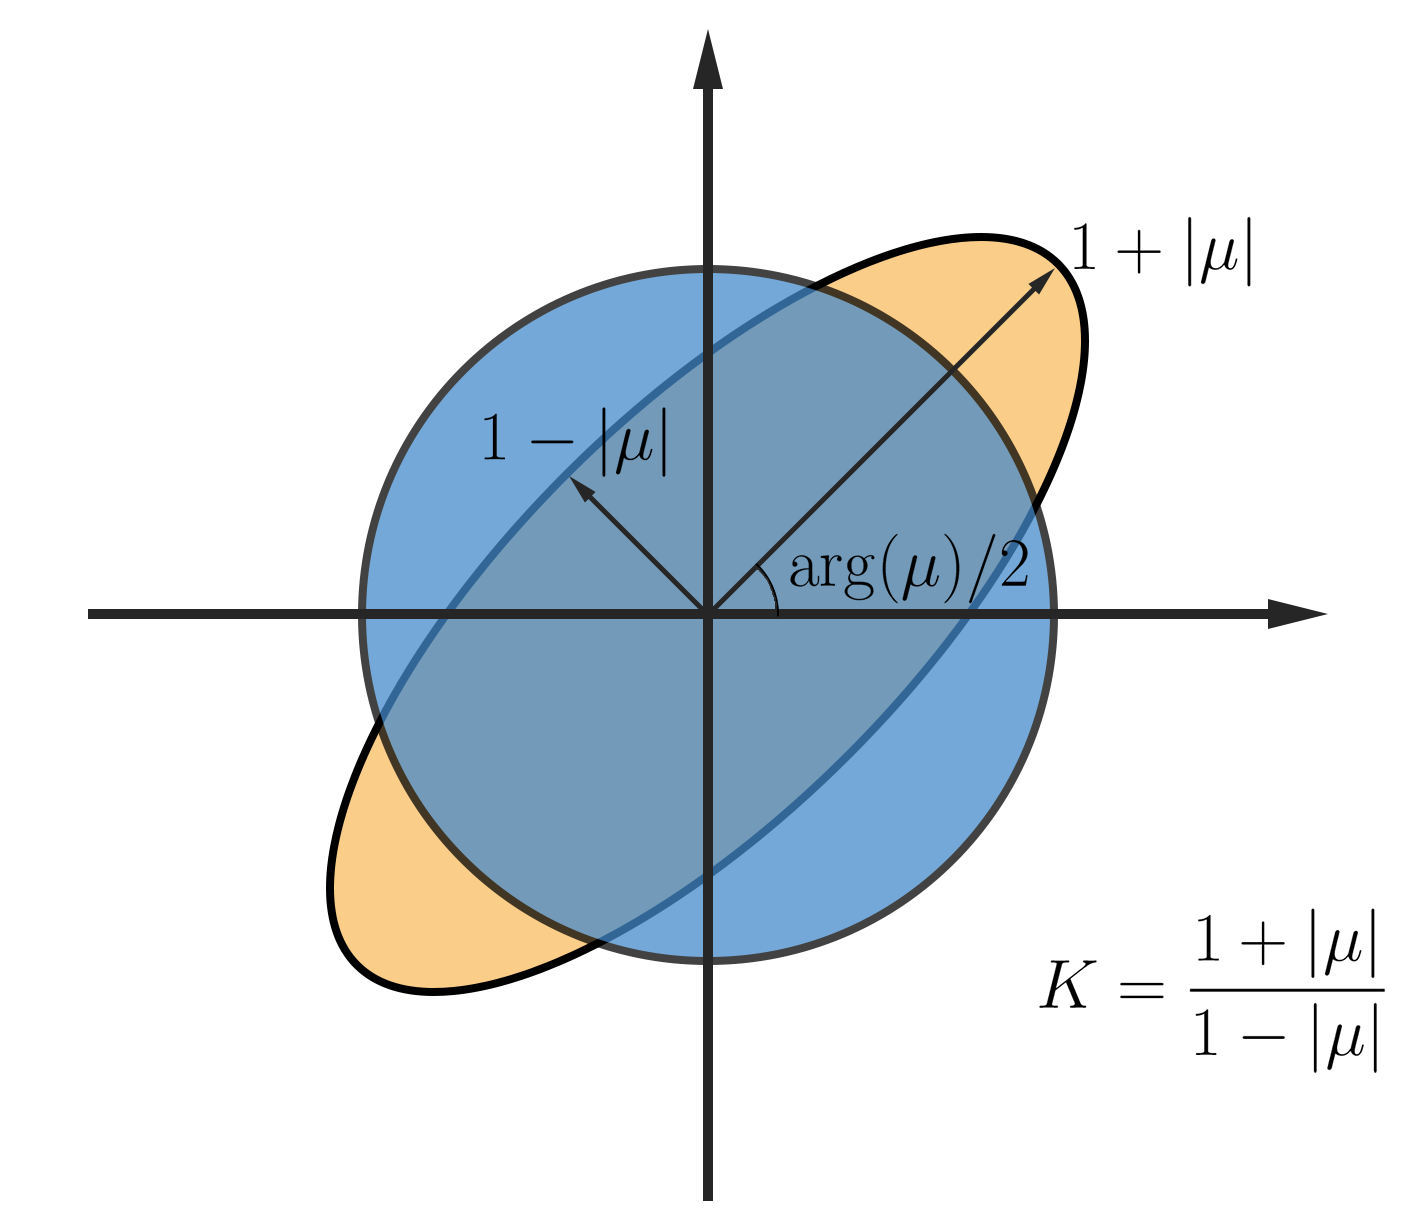
\includegraphics[width=7.6cm]{background_bc1.png}
    \end{center}
    \caption{Quasi-conformal maps infinitesimal circles to ellipses. The Beltrami coefficient measure the distortion or dilation of the ellipse under the QC map.}
    \label{fig3}
\end{figure}


Note that there is a one-to-one correspondence between the quasi-conformal mapping $f$ and its Beltrami coefficient $\mu$. Given $f$, there exists a Beltrami coefficient $\mu$ satisfying the Beltrami equation by equation (\ref{mu def}). Conversely, the following theorem states that given an admissible Beltrami coefficient $\mu$, there always exists an quasi-conformal mapping $f$ associating with this $\mu$.

\begin{theorem}[Measurable Riemannian Mapping Theorem]\label{Measurable Riemannian Mapping Theorem}
    Suppose $\mu : \C \rightarrow \C$ is Lebesgue measurable satisfying $\norm{\mu}_\infty <1$; then, there exists a quasi-conformal homeomorphism $f$ from $\C$ onto itself, which is in the Sobolev space $W_{1,2}(\C)$ and satisfies the Beltrami equation in the distribution sense. The associated quasi-conformal homeomorphism $f$ is unique up to a Mobi\"us transformation. Furthermore, by fixing $0$, $1$ and $\infty$, the $f$ is uniquely determined.
\end{theorem}

Suppose $f, g: \C \rightarrow \C$ are complex-valued function with Beltrami coefficient $\mu_f, \mu_g$ respectively. Then the Beltrami coefficient for the composition $g \circ f$ is given by 
\begin{equation}\label{mu of composition}
    \mu_{g \circ f} = \frac{\mu_f+(\mu_g \circ f) \tau}{1+\overline{\mu_f}(\mu_g \circ f) \tau},
\end{equation}
where $\tau = \frac{\overline{f_z}}{f_z}$. Note that when $g$ is conformal, $\mu_g = 0$ and 
\begin{equation}\label{mu of conformal composition}
    \mu_{g \circ f} = \mu_f.
\end{equation}

% \subsection{Conformal welding}\label{welding}
% Given a 2D bounded simply-connected shape, we can treat it as a 2D bounded simply-connected domain $\Omega \subset \C$, by Riemann mapping theorem, there exist conformal functions $\Phi_1: \D \rightarrow \Omega$ and $\Phi_2: \D^c \rightarrow \Omega^c$. $\Phi_1$ and $\Phi_2$ are unique up to a \textit{Mobi\"us transformation}:
% \begin{equation}
%     M(z) = e^{i \theta} \frac{z - a}{1 - \overline{a}z}.
% \end{equation}
% Then we can define \textit{conformal welding} as:
% \begin{equation}
%     f = \Phi_1^{-1} \circ \Phi_2.
% \end{equation}
% Such $f: \partial \D \rightarrow \partial \D$ is a diffeomorphism from $\partial \D$ to itself, which can be also thought as a periodic real-valued monotone increasing function $f_\R: [0, 2\pi) \rightarrow [0, 2\pi)$ such that $f(e^{i \theta}) = e^{i f_\R(\theta)}$ (see figure \ref{fig1}).

% However, such welding mappings are not unique because of the arbitrariness of Riemann mappings, as shown in figure \ref{unsatble}.

% \begin{figure}
%     \begin{center}
%         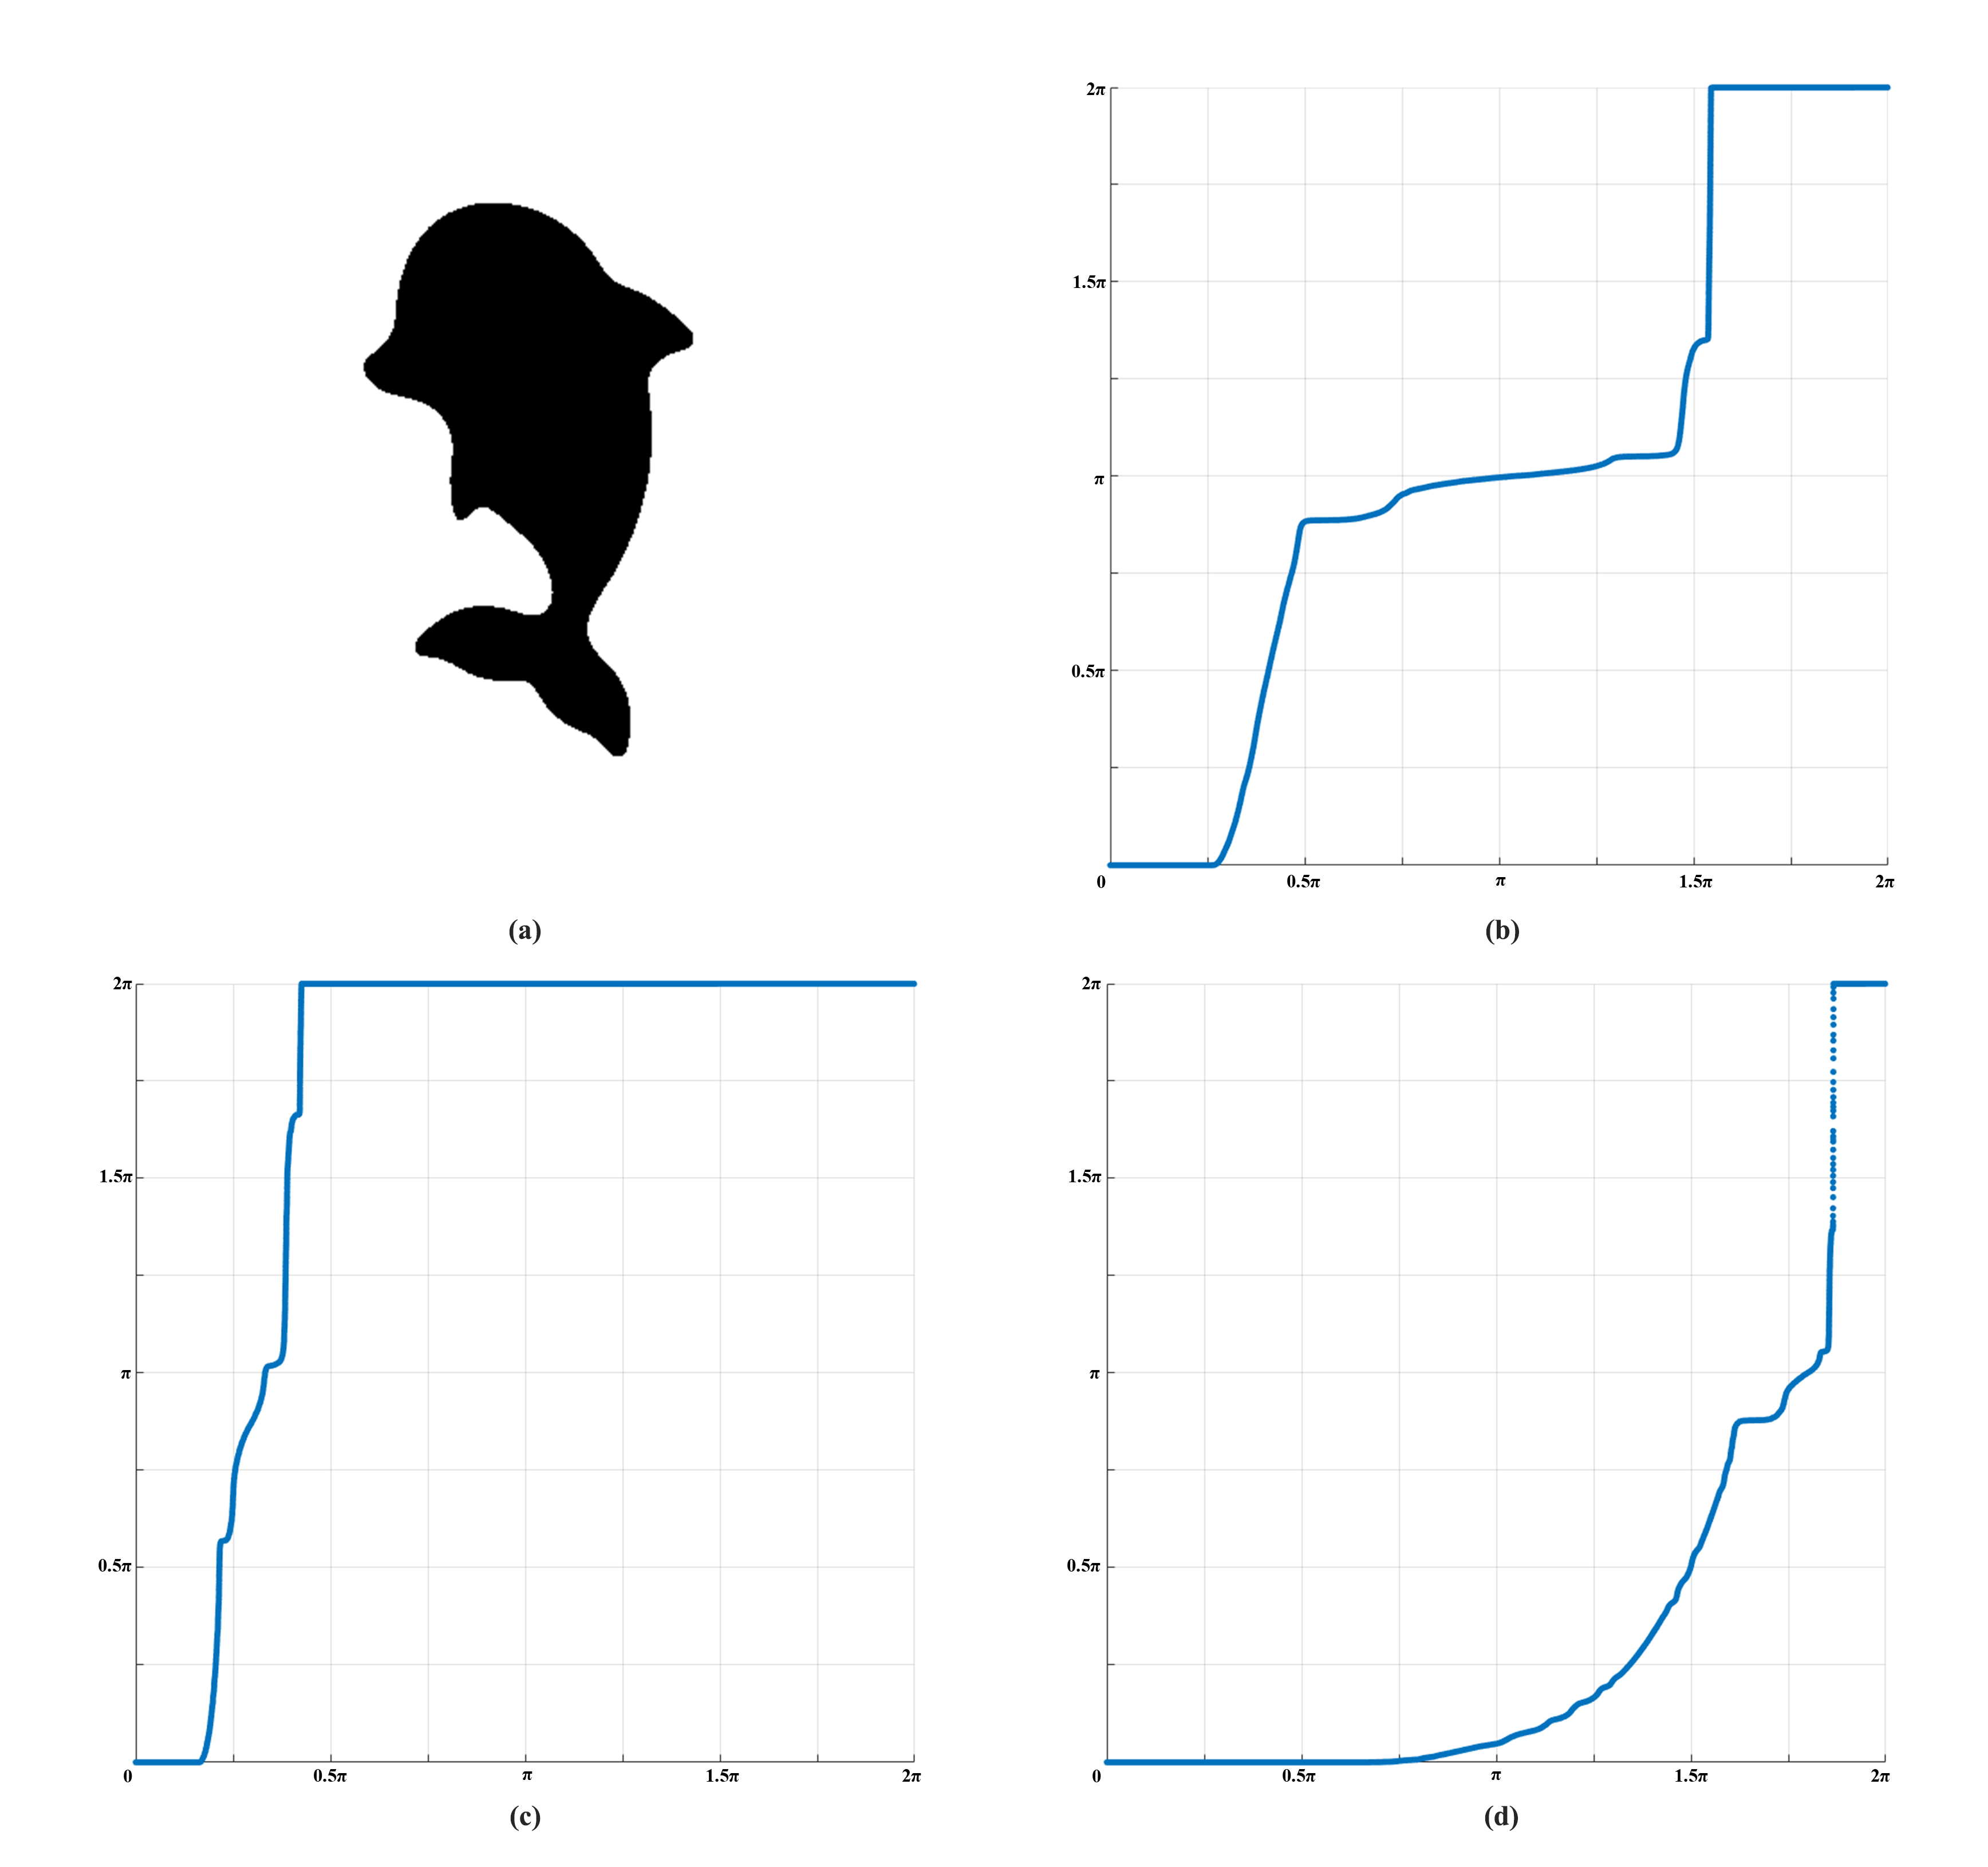
\includegraphics[width=8cm]{unstable_welding.png}
%     \end{center}
%     \caption{Different conformal welding mappings (b), (c) and (d) of the same shape (a)}
%     \label{unsatble}
% \end{figure}

% \subsection{Harmonic function and Poisson integral}
% A complex-valued function $f$ defined on $\Omega \subset \C$ is called \textit{harmonic} if it satisfies the \textit{Laplace's equation}:
% \begin{equation}
%     \Delta f = 4 \frac{\partial^2 f}{\partial z \partial \overline{z}} = \frac{\partial^2 f}{\partial x^2} + \frac{\partial^2 f}{\partial y^2} = 0,
% \end{equation}
% where $z = x + iy$, $\bar{z} = x -iy$.

% Chen \etal \cite{chen2010compositions} proved following theorem, which tells us in what condition the composition of harmonic mappings and other mappings can inherit the harmonicity.
% \begin{theorem}\label{composition of harmonic}
%     Let $f$ be a harmonic mapping, $f \circ g$ is harmonic if and only if $g(z) = az + b \overline{z} + c$, where $a$, $b$ and $c$ are constants and $g \circ f$ is harmonic if and only if $g$ is analytic or anti-analytic.
% \end{theorem}

% The harmonic function on a compact set is determined by its restriction to the boundary, which follows from the maximum principle, and the progress to find a harmonic function from the given domain and the value in domain's boundary is call \textit{Dirichlet problem}. For a special case, where the domain is unit disk, \textit{Poisson integral} shows a method to obtain the solution $H : \overline{\D} \rightarrow \C$ of Dirichlet problem from a continuous $f$ on $\partial \D$
%     \begin{equation}\label{poisson integral}
%         H(re^{i\theta}) = \frac{1}{2\pi}\int_0^{2\pi} \frac{(1-r^2)f(e^{i \varphi})}{1 - 2 r cos (\varphi - \theta) + r^2} d\varphi.
%     \end{equation}
% Such $H$ is harmonic on $\D$ and continuous on $\overline{\D}$ and has the same value with $f$ on the $\partial \D$, i.e. $H(e^{i\theta}) = f(e^{i\theta})$ (see figure \ref{harmonic}). Of course, it is uniquely determined by $f$.

% \begin{figure}
%     \begin{center}
%         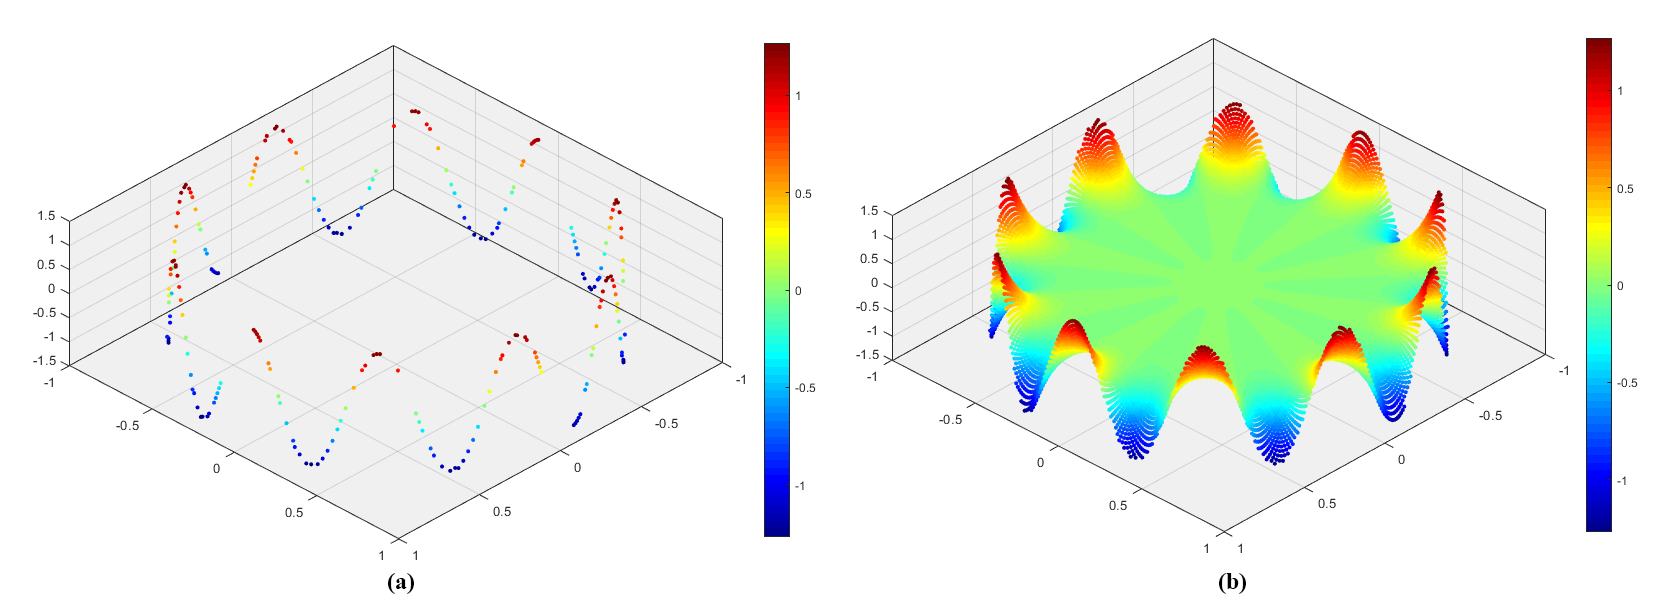
\includegraphics[width=12cm]{fig4.png}
%     \end{center}
%     \caption{(a) Continuous function $f(e^{i \theta}) = \sin(10 \theta) + \cos(10 \theta)$ defined on $\partial \D$; (b) The corresponding harmonic function $H$ generated from $f$ by the equation (\ref{poisson integral}). Note that we used real-valued function to illustrate the progress of harmonic extension for the convenience, but it is also feasible for complex-valued function.}
%     \label{harmonic}
% \end{figure}

\section{Proposed segmentation model}\label{main}
In this section, we describe our proposed shape prior segmentation model guided by HBS.

\subsection{Beltrami coefficient segmentation model}
At the beginning, we need to discribe Beltrami coefficient segmentation, which is the fundamentation of our HBS segmentation model. 

Suppose $D, D' \in \C$ are two regions, $I: D' \rightarrow \R$ is an image and $J: D \rightarrow \R$ is a binary template image. $J$ is called the \textit{topological prior image} defined as
\begin{equation}
    J(x) = \begin{cases}
        1, & x \in R,              \\
        0, & x \in D \setminus R,
    \end{cases}
\end{equation}
where $R \subset D$ is the object region of $J$. The basic idea of the segmentation model proposed by Chan \etal \cite{} is to deform this simple template $J$ to extract the target region $\Omega = f_\mu(R)$ from $I$ by a quasiconformal mapping $f_\mu: D \rightarrow D'$. Note that in most cases, $D = D'$ is a rectangle domain.

This model can be formulated as the following energy functional:
\begin{equation}\label{bc seg model}
    \min_{\mu} E_{\text{BC}}(\mu, c_1, c_2) = \min_{\mu} \int_D (I \circ f_\mu - J_{c_1,c_2})^2 + \alpha \abs{\mu}^2 + \beta \abs{\nabla \mu}^2 + \gamma \abs{u}^2 + \delta \abs{\nabla u}^2,
\end{equation}
where $u = f_\mu - Id$, $\mu: \Omega \rightarrow \C$ is the Beltrami coefficient of $f_\mu$,  $\alpha, \beta, \gamma, \delta \ge 0$ are weight parameters and $J_{c_1, c_2}$ is a generalized template image defined as
\begin{equation}
    J_{c_1, c_2}(x) = \begin{cases}
        c_1, & x \in R,              \\
        c_2, & x \in D \setminus R.
    \end{cases}
\end{equation}

The first item of $E_{\text{BC}}$ measures the difference between the deformed image $I \circ f_\mu$ and the template image $J_{c_1, c_2}$. The second item limits the magnitude of $\mu$ since $\abs{\mu} < 1$ if and only if $f_\mu$ is quasiconformal, which then ensures the bijectivity of $f_\mu$. The last three items are the regularization terms, which are used to control the smoothness of $f_\mu$.

\subsection{HBS segmentation model}
The HBS proposed in \cite{} is a powerful signature of 2D simply-connected shapes and  it represents the shape features by a complex function $B: \D \rightarrow \C$. More precisely, the HBS $B$ of the shape $\Omega_B \subset \C$ is the Beltrami coefficient of a special harmonic function $H$ such that $H(\D) = \Omega_B$. The HBS $B$ is invariant under translation, rotation and scaling, which means it can be treated as high-level shape priors with invariant geometric information under these transformations. As is well-known, translation, rotation and scaling are very common in image processing and we have good reason to believe that the HBS and the inherent invariant features it contains can effectively guide image segmentation. Inspired by this, we propose this novel HBS segmentation model.

Meanwhile, the primary objective of the segmentation model \ref{bc seg model} is to locate a suitable Beltrami coefficient $\mu$ and the corresponding quasiconformal function $f_\mu$, then the target region is $\Omega = f_\mu(R)$. 

The triplets $(B, H, \D)$ of the HBS and $(\mu, f_\mu, R)$ of model \ref{bc seg model} exhibit extreme high correlation, which implies that the HBS can be naturally integrated into this model. However, there are several differences:
\begin{enumerate}
    \item $B$ is defined on $\D$ while $\mu$ is defined on $D$. To solve this, we require $D \supset \D$ and extend $B$ to $D$ by $0$, that is
          \begin{equation}\label{mu_B}
              \mu_B = \begin{cases}
                  B, & z \in \D,              \\
                  0, & z \in D \setminus \D.
              \end{cases}
          \end{equation}
          
    \item $H$ is a quasiconformal harmonic function while $f_\mu$ is only quasiconformal. Hence we constrain the value $\Delta f_\mu$ to be very close to $0$.
          
    \item The shape can be represented as $\Omega_B = H(\D)$ in the HBS while the segmentation result is $\Omega = f_\mu(R)$ in model \ref{bc seg model}. Therefore, we fix the object region $R$ of template $J$ always to be $\D$.
\end{enumerate}

With above modifications, $\mu$ can be almost considered as a HBS. We can compare  $\mu$ and $B$ directly by $L_2$ norm $\norm{\mu - \mu_B}^2_2$. Therefore, the HBS segmentation model is formulated as follows:
\begin{equation}\label{hbs seg model}
    \begin{split}
        \min_{\mu} E_{\text{HBS}}(\mu, B, c_1, c_2) = 
        \min_{\mu} \int_D 
        & (I \circ f_\mu - J_{c_1,c_2})^2 
        + \alpha \abs{\mu}^2 + \beta \abs{\nabla \mu}^2 
        + \gamma \abs{u}^2 \\
        & + \delta \abs{\nabla u}^2
        + \lambda \abs{\mu - \mu_B}^2 + \eta \abs{\Delta u}^2.
    \end{split}
\end{equation}
The first five terms come from model \ref{bc seg model} directly and play the same roles as before. The sixth term measures the similarity of $\mu$ and $B$. And the last term with a big penalty parameter $\eta$ is a soft constrain that $f_\mu$ is harmonic.

The term $\int_D \abs{\mu - \mu_B}^2$ is crucial for model \ref{hbs seg model}. Note that the template $J$ is fixed, the HBS $B$ contains all shape prior informations by this term. $B$ is corresponding to a unique shape $\Omega_B$ up to translation, rotation and scaling. The smaller this term is, the more similar the segmentation result $\Omega = f_\mu(\D)$ and $\Omega_B$ are, which provides a simple yet effective method to utilize prior information for guiding the segmentation process.

The existence of the minimizer of model \ref{hbs seg model} over $\mu$ is guaranteed by the following theorem.
\begin{theorem}\label{existence}
    The energy functional $E_{\text{HBS}}$ in model \ref{hbs seg model} has a minimizer in $\mathcal{A}^M_\epsilon \subset C^1(D)$, where
    \begin{equation*}
        \mathcal{A}^M_\epsilon = \{ \mu \in C^1(D) : \norm{D \mu}_\infty \le M, \norm{\mu}_\infty \le 1 - \epsilon \},
    \end{equation*}
    for some $M > 0$ and $\epsilon \in (0, 1)$.
\end{theorem}

\begin{proof}
    Following a similar argument in \cite{}, we can show that $\mathcal{A}^M_\epsilon$ is Cauchy complete and totally bounded, and hence compact. The three terms containing $\mu$, $\int_D \abs{\mu}^2$, $\int_D \abs{\nabla \mu}^2$ and $\int_D \abs{\mu - \mu_B}^2$, are obviously continuous over $\mu$. Also, according to the Beltrami holomorphic flow and Bojarski theorem, the associated quasiconformal map $f_\mu$ varies continuously (smoothly) under a continuous (smooth) variation of $\mu$. Hence, the other four terms are continuous over $\mu$ as well. Since $E_\text{HBS}$ is continuous on the compact set $\mathcal{A}^M_\epsilon$, $E_\text{HBS}$ has a minimizer in it.
\end{proof}

Similar with that mentioned in \cite{}, the smaller $\epsilon$ is, the more geometric distortion is allowed, and the deformed contour get closer to real object boundary. However, small $\epsilon$ increses the difficulty to find the minimizer, which is a trade-off between the accuracy and the efficiency. Meanwhile, the bigger $M$ is, the smoother the deformed contour is, but we get less accurate segmentation result. We can choose $\epsilon$ and $M$ according to the prior information of the given shape.

\section{Numerical algorithm}
In practice, a digital image consists of many pixels and can be discreted by a triangular mesh $(V, E, F)$, where $V \subset D$ is the set of vertices, $E$ is the set of edges between vertices and $F$ is the set of triangle faces formed by edges. The deform function $f_{\mu_V}: V \rightarrow D$ is piecewise linear on each face and $f_{\mu_V}|_{\partial D} = Id$. The first derivative of $f_{\mu_V}$ is piecewise constant and so the Beltrami coefficient $\mu_F: F \rightarrow \C$ is a constant on each face. Then we compute $\mu_V: V \rightarrow \C$ by taking the average of $\mu_F$ on the faces sharing the same vertex. We do the same thing to get $\mu_{B,V}$. Although the input images are only defined on $V$, we treat it as a continuous functions $I, J: D \rightarrow \R$ through interpolation for the sake of convenience in the discussion. Hence, the deformed image $I \circ f_{\mu_V}: V \rightarrow \R$ can be achieved. As the result, the discrete HBS segmentation model is as follows:
\begin{equation}\label{discrete hbs seg model}
    \begin{split}
        \min_{\mu_V} E_{\text{DHBS}}(\mu_V, B, c_1, c_2) = 
        \min_{\mu_V} \sum_{v \in V}
        & (I \circ f_{\mu_V} - J_{c_1,c_2})^2 
        + \alpha \abs{\mu_V}^2 + \beta \abs{\nabla \mu_V}^2 
        + \gamma \abs{u_V}^2 \\
        & + \delta \abs{\nabla u_V}^2
        + \lambda \abs{\mu_V - \mu_{B,V}}^2 + \eta \abs{\Delta u_V}^2.
    \end{split}
\end{equation}

However, this model implies a constraint, $\mu_V = \frac{\partial f_{\mu_V}}{\partial \bar{z}} / \frac{\partial f_{\mu_V}}{\partial z}$, which presents a significant challenge during searching the minimizer. To solve this, we disconnect the strong coupling between $\mu_V$ and $f_{\mu_V}$ and set another Beltrami coefficient $\nu_{V}$ without direct relation with $f_{\mu_V}$ as an alternative, which induces a weak HBS segmentation model:
\begin{equation}\label{weak discrete hbs seg model}
    \begin{split}
        \min_{\mu_V, \nu_V} E_{\text{WHBS}}(\mu_V, \nu_V, B, c_1, c_2) = 
        & \min_{\mu_V, \nu_V} \sum_{v \in V}
        (I \circ f_{\mu_V} - J_{c_1,c_2})^2 
        + \alpha \abs{\nu_V}^2 + \beta \abs{\nabla \nu_V}^2 
        + \gamma \abs{u_V}^2 \\
        & + \delta \abs{\nabla u_V}^2
        + \lambda \abs{\nu_V - \mu_{B,V}}^2 + \eta \abs{\Delta u_V}^2 + \tau \abs{\nu_V - \mu_V}^2.
    \end{split}
\end{equation}
Here we replace all $\mu_V$ by $\nu_V$ in 2rd, 3th and 6th terms of model \ref{discrete hbs seg model} and add a new term $\tau \abs{\nu_V - \mu_V}^2$ to handle the difference between $\mu_V$ and $\nu_V$, where $\tau > 0$ is a big penalty parameter. If $\nu_V = \mu_V$, $E_{\text{WHBS}}$ will degenerate to $E_{\text{DHBS}}$. This modification allows us to split the original problem into 2 parts and we call them \textbf{$\mu$ subproblem}
\begin{equation}\label{mu subproblem}
    \min_{\mu_V} E_{\mu}(\mu_V, c_1, c_2) = 
    \min_{\mu_V} \sum_{v \in V}
    (I \circ f_{\mu_V} - J_{c_1,c_2})^2 
    + \gamma \abs{u_V}^2 
    + \delta \abs{\nabla u_V}^2
    + \eta \abs{\Delta u_V}^2,
\end{equation}
and \textbf{$\nu$ subproblem}
\begin{equation}\label{nu subproblem}
    \min_{\nu_V} E_{\nu}(\mu_V, \nu_V, B) = 
    \min_{\nu_V} \sum_{v \in V}
    \alpha \abs{\nu_V}^2 + \beta \abs{\nabla \nu_V}^2 
    + \lambda \abs{\nu_V - \mu_{B,V}}^2 + \tau \abs{\nu_V - \mu_V}^2.
\end{equation}

After such separation, these two subproblem has gained clearer and more practical meanings. The core of $\mu$ subproblem is to find the deform map $f_{\mu_V}$ according to the pixel level difference as well as other regularizations, then $\mu_V$ is achieved naturally. While the target of $\nu$ subproblem is to normalize the Beltrami coefficient $\mu_V$ from the last step under shape prior information for further segmentation. The soft constrain term $\abs{\nu_V - \mu_V}$ is the bridge to connect these two processes. Therefore, we can solve subproblems alternatively until they converge, which then gives the solution of original optimization problem \ref{discrete hbs seg model}. More specifically, suppose $\mu_{V,n}$ and $\nu_{V,n}$ is obtained in $n$-th iteration, then $\mu_{V,n+1}$ and $\nu_{V,n+1}$ can be computed by
\begin{equation}
    \mu_{V,n+1} = \argmin_{\mu_V} E_\mu(\mu_V, c_1, c_2),
\end{equation}
\begin{equation}
    \nu_{V,n+1} = \argmin_{\nu_V} E_\nu(\mu_{V,n+1},\nu_V, B).
\end{equation}
The total algorithm is summarized in algorithm \ref{main alg}.

\subsection{Solving $\mu$ subproblem}
Note that there are the other two input variables $c_1$ and $c_2$ in $E_\mu$. Compared to solving for multiple variables simultaneously, a simpler and more common choice is to determine them in advance. Given $f_{\mu_{V,n}}$, it can be regarded as another optimization problem and we can compute the minimizers explicitly by
\begin{equation}\label{mu c1 c2}
    c_1 = \frac{\sum_{v \in V \cap \D} I \circ f_{\mu_{V,n}}}{\sharp (V \cap \D)}, \quad
    c_2 = \frac{\sum_{v \in V \setminus \D} I \circ f_{\mu_{V,n}}}{\sharp (V \setminus \D)},
\end{equation}
where $\sharp$ means the number of vertices inside the set. Except in necessary cases, we will omit all occurrences of $c_1$ and $c_2$ in the following discussion.

Even theorem \ref{existence} ensure the existence of minimizer, excessively large deformations can still burden the algorithm, leading to fluctuating segmentation results and long computation time. Instead of directly calculating $f_{\mu_{V,n+1}}$, we attempt to compute a smaller deformation based on the previous segmentation result and use a sequence of small deformations to represent the desired $f_{\mu_{V,n+1}}$
\begin{equation}
    f_{\mu_{V,n+1}} = g_{n+1} \circ f_{\mu_{V,n}} = g_{n+1} \circ \cdots \circ g_1 \circ f_{\mu_{V,0}},
\end{equation}
where $g_k: D \rightarrow D$. Since $f_{\mu_{V,n}}$ is quasiconformal then bijective, $f_{\mu_{V,n}}^{-1}$ exists, we  have
\begin{equation}\label{mu 1st term approx v}
    \sum_{v \in V} (I \circ g_{n+1} \circ f_{\mu_{V,n}} - J)^2
    = \sum_{v \in f_{\mu_{V,n}}(V)} (I \circ g_{n+1} - J \circ f_{\mu_{V,n}}^{-1})^2 
    \approx \sum_{v \in V} (I \circ g_{n+1} - J_n)^2,
\end{equation}
where $J_n = J \circ f_{\mu_{V,n}}^{-1}$ is the deformed template image by $f_{\mu_{V,n}}$ and is the temporary segmentation result of the last iteration. The approximate equality is due to the acceptable interpolation error, which will decreases as the image resolution increases. Furthermore, this term can be expanded by a first-order Taylor series
\begin{equation}\label{mu 1st term taylor}
    \sum_{v \in V} (I \circ g_{n+1} - J_n)^2 
    \approx \sum_{v \in V} \abs{I - J_n + \nabla I \cdot h_{n+1}}^2,
\end{equation}
where $h_{n+1} = g_{n+1} - Id$. 

Since $u_{V,n+1} = (h_{n+1} - f_{\mu_{V,n}}^{-1} + Id) \circ f_{\mu_{V,n}}$, the same interpolation approximation in \ref{mu 1st term approx v} can be also applied to the other regular terms of $E_\mu$ in \ref{mu subproblem}. Finally, $\mu$ subproblem can be rewritten as:
\begin{equation}
    \min_h E_\mu (h, J)
    = \min_h \sum_{v \in V} \abs{I - J + \nabla I \cdot h}^2 
    + \gamma \abs{h}^2
    + \delta \abs{\nabla h}^2 
    + \eta \abs{\Delta h}^2.
\end{equation}
The minimizer satisfies following PDE according to Euler-Langrange equation
\begin{equation}\label{mu problem pde}
    (I-J) \nabla I + \nabla I^2 \cdot h + \gamma h - \delta \Delta h + \eta \Delta^2 h = 0,
\end{equation}
subject to $h = 0$ on $\partial D$. We mark the solution of \ref{mu problem pde} as $h_{n+1}$ and the deform function is
\begin{equation}\label{mu deform function f}
    f^*_{\mu_{V,n+1}} = (h_{n+1} + Id) \circ f_{\mu_{V,n}}.
\end{equation}
Then the Beltrami coefficient $\mu_{V,n}$ can be computed on the triangular mesh by
\begin{equation}\label{mu mu}
    \mu_{V,n+1}(v) = \frac{\partial f^*_{\mu_{V,n+1}}}{\partial \bar{z}}(v) \bigg / \frac{\partial f^*_{\mu_{V,n+1}}}{\partial z}(v),
\end{equation}
To avoid some numerical errors, we designate $\mu_{V,n}(v) = 0$ if $\frac{\partial f^*_{\mu_{V,n}}}{\partial z}(v) = 0$ for some $v \in V$.

Besides, we also need $\abs{\mu_{V,n}(v)} < 1$ for all $v \in V$ to guarante the deform function is quasiconformal, so an additional truncation $T$ is applied to those points that are to large as
\begin{equation}\label{mu truncate}
    T(\mu)(v) = \begin{cases}
        \mu(v),                                  & \abs{\mu(v)} < 1 - \epsilon,    \\
        \frac{1 - \epsilon}{\abs{\mu(v)}}\mu(v), & \abs{\mu(v)} \ge 1 - \epsilon,
    \end{cases}
\end{equation}
where $\epsilon$ is a small positive number. So far, we have addressed $\mu$ subproblem and obtained the desired $\mu_{V,n+1}$.

\subsection{Solving $\nu$ subproblem}
As mentioned before, $\nu$ subproblem \ref{nu subproblem} essentially involves refining the solution $\mu_{V,n+1}$ obtained from the previous step. We apply the Euler-Langrange equation to $E_\nu$ with respect to $\nu_V$:
\begin{equation}\label{nu problem pde}
    \alpha \nu_V - \beta \Delta \nu_V + \lambda (\nu_V - \mu_{B,V}) + \tau (\nu_V - \mu_{V,n+1}) = 0,
\end{equation}
subject to $\nu_V = 0$ on $\partial D$. The result of this PDE is $\nu_{V,n+1}$, which solves subproblem \ref{nu subproblem}. Note that we also truncate it by $T$ as \ref{mu truncate}.

By LBS method, we reconstruct the corresponding refined deform function $f_{\mu_{V,n+1}}$ from $\nu_{V,n+1}$ with boundary condition $f_{\mu_{V,n+1}} = Id$ on $\partial D$. It, rather than the $f_{\mu_{V,n+1}}^*$ in \ref{mu deform function f}, induces the temporary segmentation result $J_{n+1} = J \circ f_{\mu_{V,n+1}}^{-1}$ and then is used in next iteration.


\begin{algorithm}[H]
    \caption{HBS segmentation algorithm}
    \label{main alg}
    \begin{algorithmic} 
        \STATE \textbf{Inputs:} Rectangle domain $D \subset \C$, the image to be segmented $I: D \rightarrow \R$, unit disk template $J: D \rightarrow \R$, HBS $B: \D \rightarrow \C$, max iteration times $N$, stop precision $\epsilon$ and other model parameters.
        \STATE \textbf{Initialize:} Build triangle mesh $(V, E, F)$ on $D$ and compute $\mu_{B,V}$ form $B$.
        \STATE Let $n=1$ and $f_{\mu_{V,1}} = Id$.
        \WHILE{$n < N$}
        \STATE Compute $c_1$ and $c_2$ by \ref{mu c1 c2} and then $J_n = J \circ f_{\mu_{V,n}}$.
        \STATE Solve \ref{mu problem pde} and get $h_{n+1}$.
        \STATE Compute $f^*_{\mu_{V,n+1}}$ by \ref{mu deform function f}.
        \STATE Compute $\mu_{V,n+1}$ by \ref{mu mu}.
        \STATE Solve \ref{nu problem pde} and get $\nu_{V,n+1}$.
        \STATE Compute $f_{\mu_{V,n+1}}$ by LBS method.
        \IF{$\norm{f_{\mu_{V,n+1}} - f_{\mu_{V,n}}}_2 < \epsilon$}
        \STATE Break.
        \ENDIF
        \STATE Let $n = n+1$.
        \ENDWHILE
        \RETURN Segmentation result $f_{\mu_{V,n+1}}(\D)$.
    \end{algorithmic}
\end{algorithm}



\section{Experimental result}\label{resul}
In this section, we demonstrate the effectiveness of the proposed HBS segmentation model through different experimental results. Our experiments are implemented using MATLAB R2014a running on 4-way Intel(R) Xeon(R) Gold 6230 processors with 80 cores at 2.10GHz base frequency and 1024 GB RAM under Ubuntu 18.04LTS 64-bit operating system.

\subsection{Binary images}
Deformation of the target object due to various reasons such as image corruption, object occlusion, etc., is very common. In such cases, prior information can greatly assist us in making accurate segmentations. By utilizing HBS as the prior, the proposed segmentation model is aware of the approximate shape of the target object beforehand, leading to improved performance. 

To illustrate this more intuitively, we have constructed a series of simple binary images to validate our model and display the results in Figure \ref{exp1}. For each row, the 1st column is the original shape, the 2nd column is the template shape, the 3rd column is the HBS corresponding to the template shape, the 4th column is the segmentation result without HBS and the 5th column is the segmentation result of our proposed model. Before analyzing the results, it is important to clarify some points and we will use them in the following experiments unless otherwise specified.
\begin{enumerate}
    \item The template provided in the 2nd column is not the $J$ in our model, which has been fixed as the unit disk. Here the template shape is solely used to compute HBS and will not be fed into the model. We show them to help our humans to have a visual understanding of the prior information.
    \item Exactly speaking, it is the magnitude of $\mu_{B,V}$ shown in the 3rd column.
    \item The green line in 4th and 5th column is the segmentation boundary.
    \item The segmentation result without HBS is obtained by setting $\lambda = \eta = 0$ of model \ref{hbs seg model}, which then is equivalent to the Beltrami coefficient segmentation model \ref{bc seg model}. We also use the unit disk as $J$.
\end{enumerate}

Let's look back on Figure \ref{exp1}, from which we can preliminarily obtain the following information:
\begin{enumerate}
    \item The HBS played a significant role in the low-quality image segmentation. We made some modifications to basic geometric shapes, resulting in them lacking certain parts or having additional parts. Under the guidance of HBS, our model essentially disregarded the impact of these variations and provided satisfactory segmentation, which almost matched the given template. While the segmentation result without HBS is much more faithful to the actual shape boundaries.
    \item The proposed model can segment both the simply-connected and multi-connected images and then give simply-connected results. Although the HBS is the signature of simply-connected shapes, our model works well on multi-connected images in 3rd and 4th rows.
    \item The proposed model does not impose any requirements on the position, size, or orientation of the target object in the image. The HBS is invariant under translation, rotation and scaling and our model inherited this feature. With the same HBS, 1st and 2nd row are rectangles in different size and our model can segment them correctly. Similarly, 3rd and 4th rows are triangles in different orientation.
    \item The proposed model tolerates reasonable discrepancies between the prior information and the actual image. In the 5th row, the segmentation result is acceptable when the template is a circle and the image is close to a ellipse.
    \item The proposed model effectively utilizes the prior information provided by the given template rather than simply extracting some basic geometric properties. In 2rd row, our model handle convex and concave parts at the same time. We will further demonstrate this in the following experiment.
\end{enumerate}

\begin{figure}
    \begin{center}
        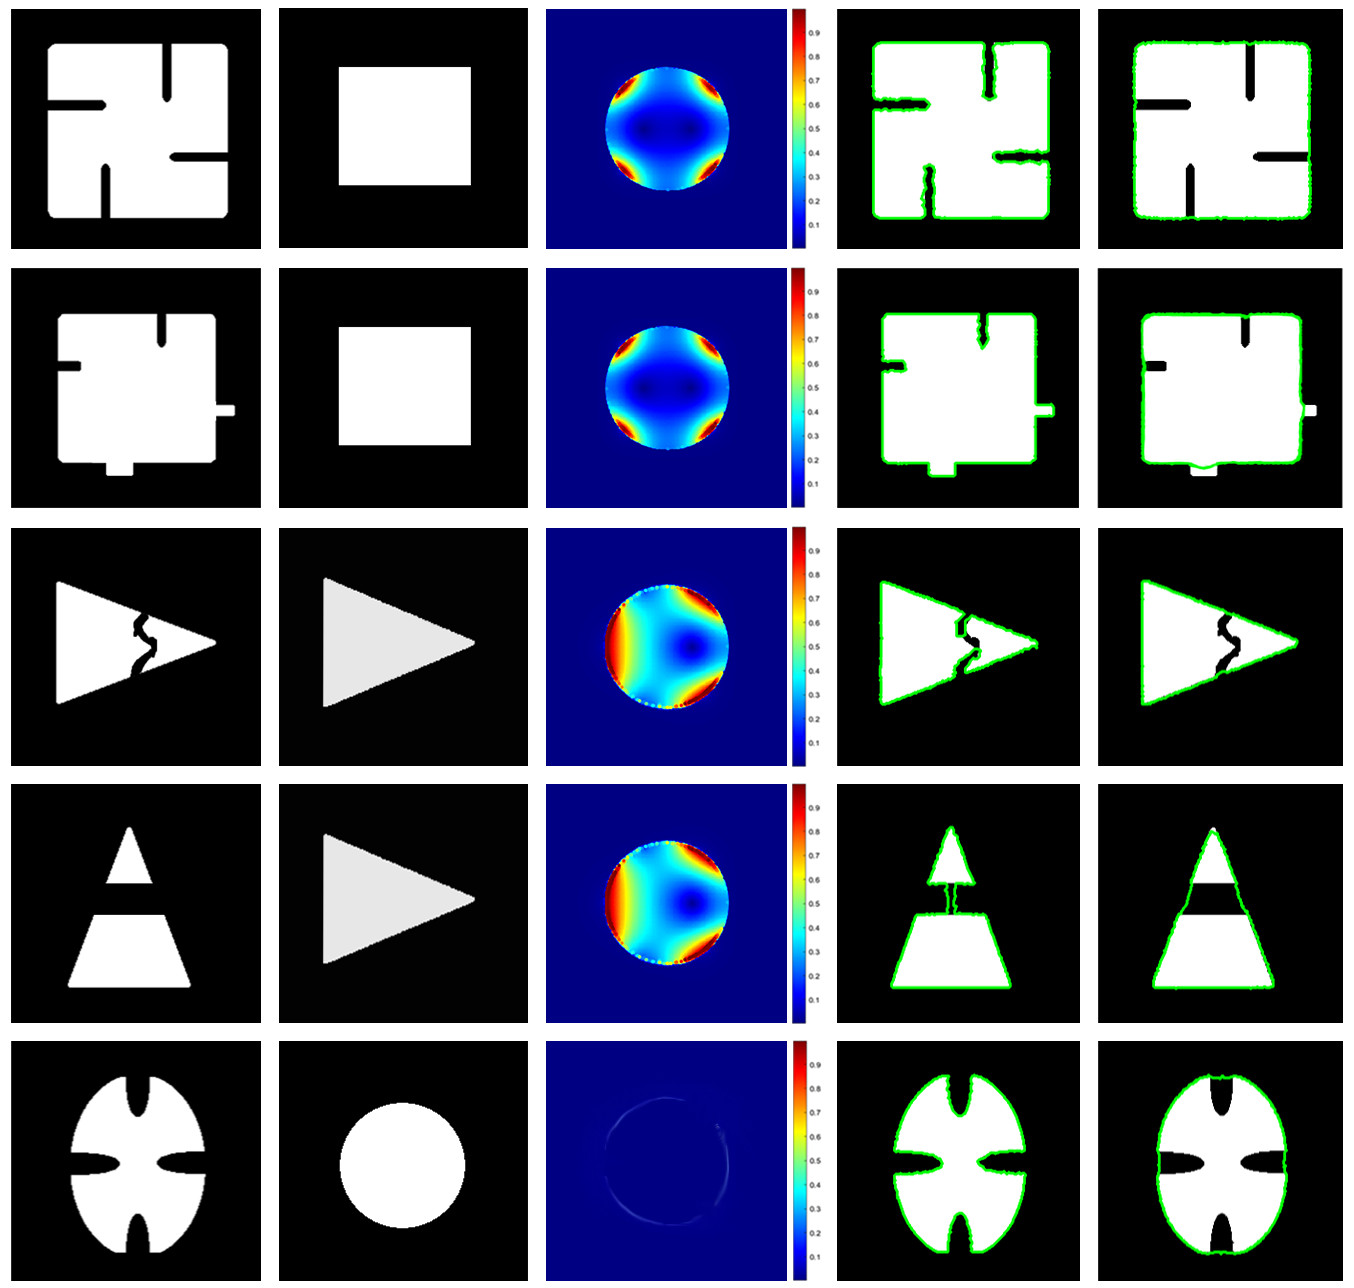
\includegraphics[width=15.5cm]{src/exp1.png}
    \end{center}
    \caption{Segmentation results of binary images.}
    \label{exp1}
\end{figure}

We will further observe the impact of different templates on the segmentation results from Figure \ref{exp2}. The meanings of each column is the same with Figure \ref{exp1}. The original image is similar to a hexagon, and we used hexagon, circle, diamond and square templates to segment it, with the results shown in 1st, 2nd, 3rd and 4th row respectively. We can find that all of the segmentation results preserve some shape characteristics of their corresponding templates but their performances differ significantly. The 1st row is the best, 2nd row is still acceptable but 3rd and 4th rows are far from accurate. That indicates our proposed method is highly sensitive to the given template. A precise template gives a prefect segmentation result, while an unsuitable template leads a terrible one. But on the other hand, it also implies our model has a certain level of understanding of the prior information.

\begin{figure}
    \begin{center}
        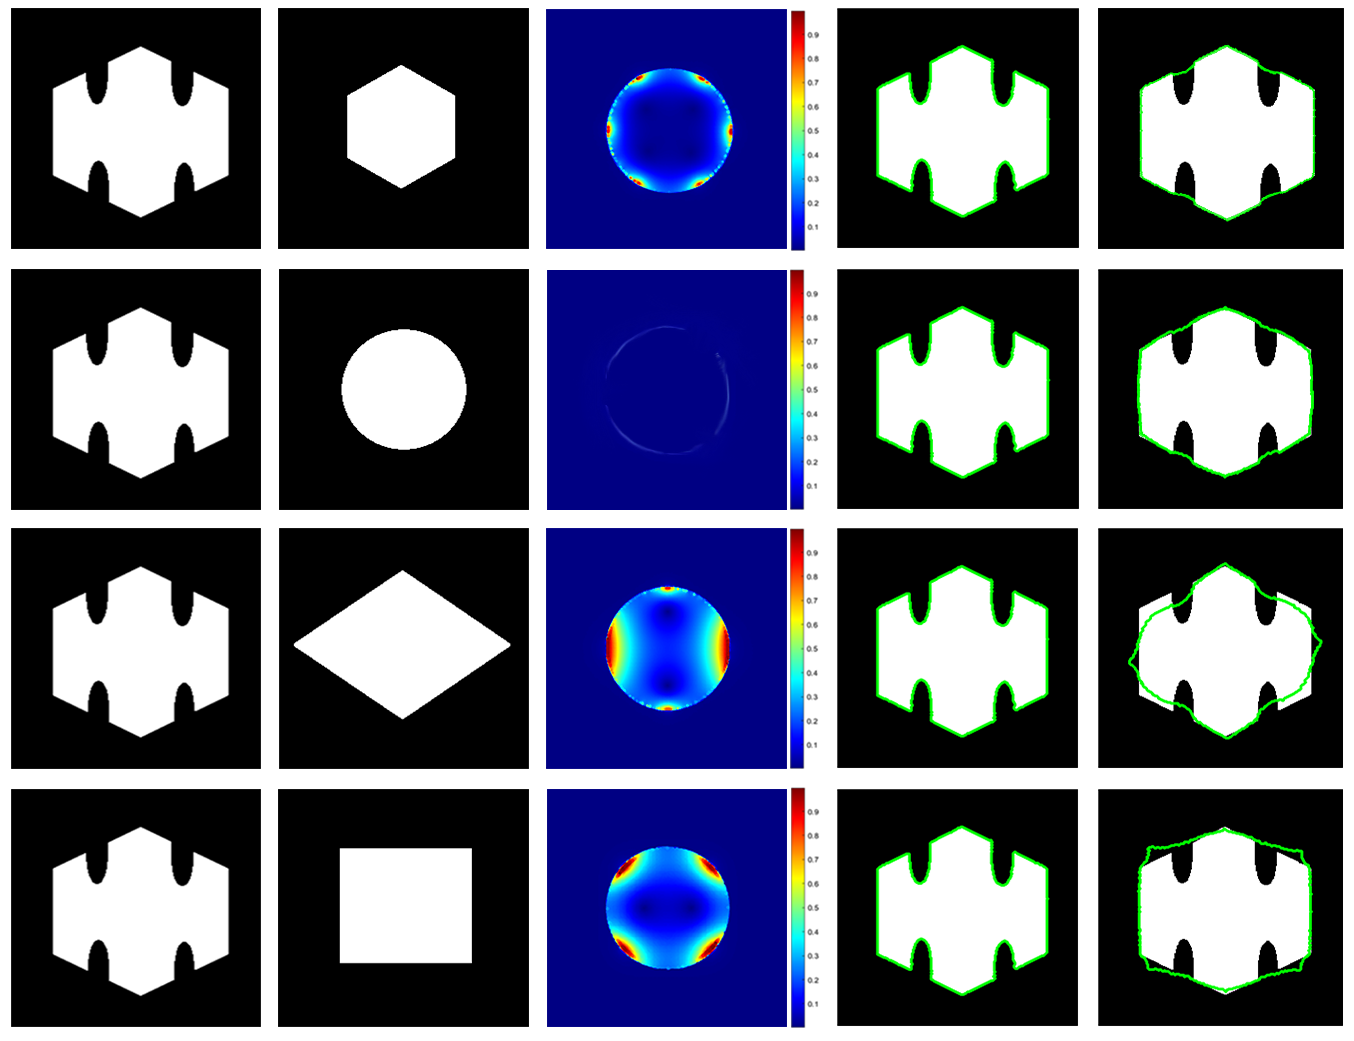
\includegraphics[width=15.5cm]{src/exp2.png}
    \end{center}
    \caption{Segmentation results under different templates.}
    \label{exp2}
\end{figure}

\subsection{Natural images}
The experimental results on binary images demonstrate that our model can effectively utilize prior information to segment partially damaged target object. However, we are far from satisfied with this and we extend the model's application to real-world images.

Figure \ref{exp3} presents some results on natural images. As before, original image, template, HBS, segmentation without HBS and segmentation with HBS are sequentially displayed in columns 1 to 5 of each row. The 1st row is a grayscale image with a bear in grass. Without HBS, the model only relies on the intensity of grayscale values to determine the shape boundaries, which results in the top boundary being limited to the brighter nose and forehead, while the bottom boundary appears jagged due to the grass. When HBS is specified, even the circle is not a very suitable template, it helps our proposed HBS segmentation model to generate a much smoother and more complete result. The other 3 images are color images, which need to be compressed RGB to grayscale before applying our model. The result in 2nd row demonstrates no matter how many pieces the target object is seprated to, our model can segment it as a simply-connected entity, just like what it does on binary images. The 3rd row represents similar but a more practical scenario, occlusion, and our model successfully and accurately identifies the white paper behind pens. In the 4th row, our model also completely locates the signboard partially covered under the dust. 

\begin{figure}
    \begin{center}
        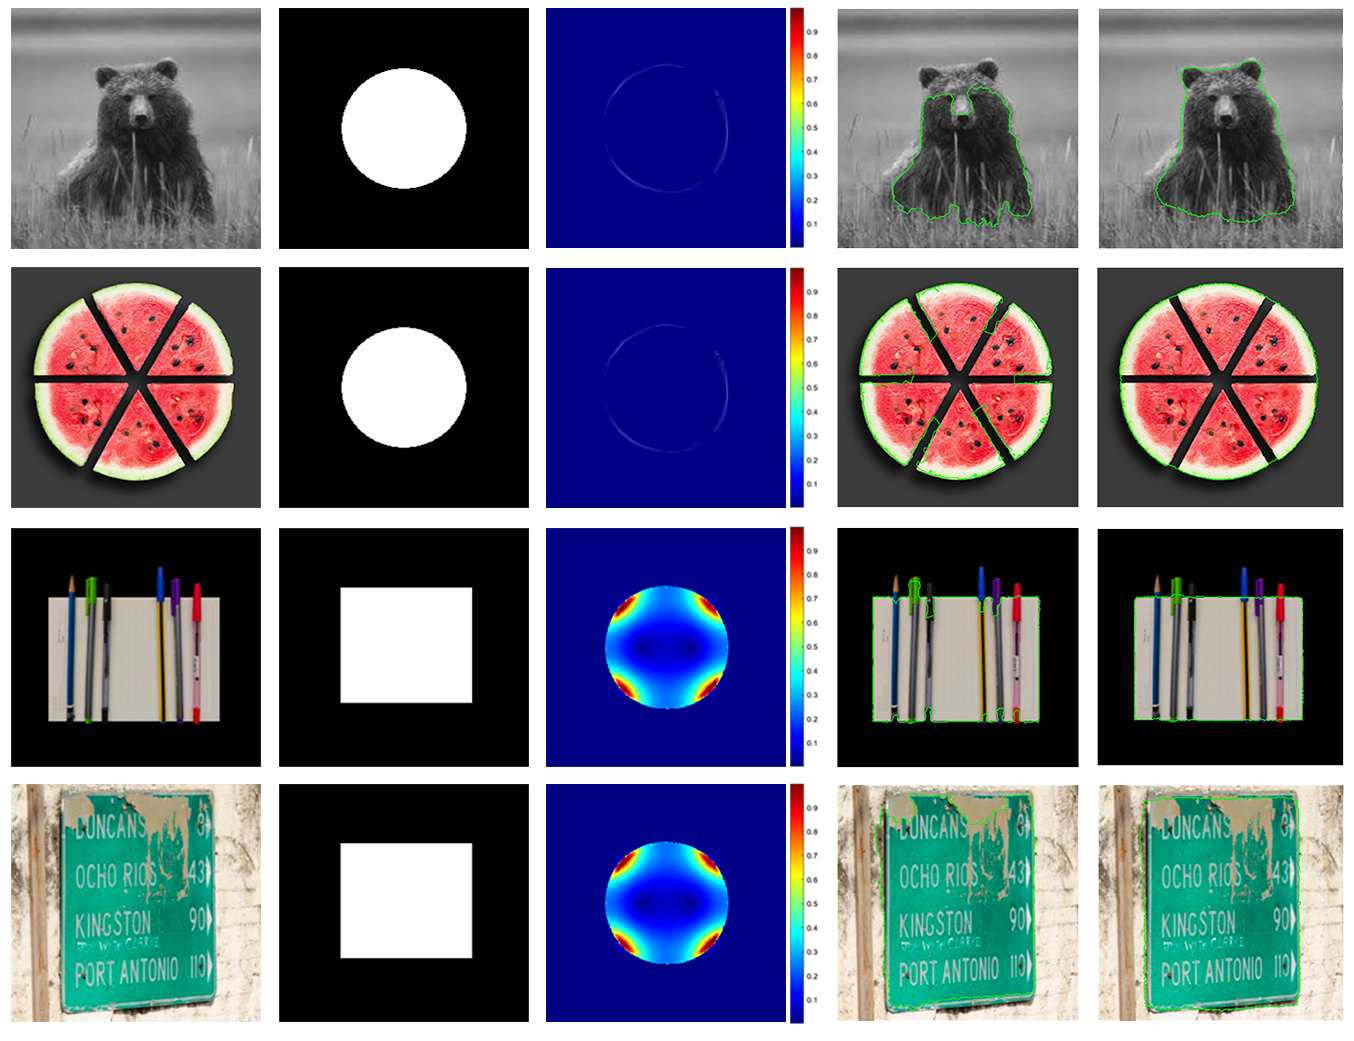
\includegraphics[width=15.5cm]{src/exp3.png}
    \end{center}
    \caption{Segmentation results of natural images.}
    \label{exp3}
\end{figure}



\section{Conclusion}\label{conclusion}

\bibliographystyle{siamplain}       % APS-like style for physics
\bibliography{cite}
% Non-BibTeX users please use
% \begin{thebibliography}{}
% %
% % and use \bibitem to create references. Consult the Instructions
% % for authors for reference list style.
% %
% \bibitem{RefJ}
% % Format for Journal Reference
% Author, Article title, Journal, Volume, page numbers (year)
% % Format for books
% \bibitem{RefB}
% Author, Book title, page numbers. Publisher, place (year)
% % etc
% \end{thebibliography}

\end{document}
